% Provenance (never printed): see sources/outline_sources.md (Year 2: fractional
% crystallisation, Bowen's series, compatible and incompatible elements, mixing and
% assimilation, layered intrusions).
% Curves from figdata/bachelor-2/differentiation.py (Bowen 1913 plagioclase loop, Rayleigh and
% equilibrium laws, Wilcox 1954 Paricutin analyses and mass balance, AFC closed form,
% Tegner et al. 2023 Skaergaard whole-rock data); exercise and problem values in the Book 4
% scratch calculator calc/ch08.py.
\chapter{Magmatic Differentiation}\label{ch:b2:magmatic-differentiation}

On 20 February 1943 a volcano began to erupt in the west of Mexico, and it went on
for nine years. Its first lavas were basaltic andesites with \qty{55}{\percent}
silica; its last, in February 1952, were andesites with slightly over
\qty{60}{\percent}. The volcano, Parícutin, did not move to another source in the
meantime, and its lavas were analysed one after the other as they came out. The
\omterm{def:b2:magma-emplacement:magma}{magma} beneath it changed itself: it grew crystals and left them behind, and it ate
some of the granitic rock around it. A \omterm{def:b2:magma-emplacement:magma}{magma} that leaves the mantle as a basalt can
end as a rhyolite, and the rocks it leaves behind on the way record how it did so.
This chapter follows a \omterm{def:b2:magma-emplacement:magma}{magma} as it cools: the order in which minerals crystallise,
the laws that tell how major and \omterm{def:b2:elements-in-the-earth:trace}{trace elements} change when crystals are removed,
the rocks built from those crystals, and what happens when the \omterm{def:b2:magma-emplacement:magma}{magma} takes in
another \omterm{def:b2:magma-emplacement:magma}{magma} or the crust.
% ledger: wilcox54:paricutin

\begin{recall}
\textbf{From the high-school volume}: igneous rocks and their textures; the order
in which minerals crystallise from a basaltic \omterm{def:b2:magma-emplacement:magma}{magma}, olivine first and quartz last,
found by Bowen's experiments. \textbf{From the chemistry books' Year 2 volume}:
binary phase diagrams, solid solutions and the lever rule. \textbf{From the Year 1
volume}: plagioclase, a solid solution between anorthite \ce{CaAl2Si2O8} and albite
\ce{NaAlSi3O8}, and the other rock-forming silicates; thin sections between crossed
polars. \textbf{From \cref{ch:b2:elements-in-the-earth}}: the mineral--melt and bulk
partition coefficients, $\bar D = \sum_i x_i D_i$, compatible and \omterm{def:b2:elements-in-the-earth:partition}{incompatible
elements}, \omterm{def:b2:elements-in-the-earth:normalised}{normalised diagrams} and the \omterm{prop:b2:elements-in-the-earth:normalised}{europium anomaly}. \textbf{From
\cref{ch:b2:isotope-geochemistry}}: isotope ratios as tracers and the \omterm{prop:b2:isotope-geochemistry:mixing}{mixing
hyperbola}. \textbf{From \cref{ch:b2:mantle-melting}}: the diopside--anorthite
eutectic, \omterm{def:b2:mantle-melting:peritectic}{incongruent melting}, ternary diagrams and \omterm{def:b2:mantle-melting:primary}{primary magmas}.
\end{recall}

\section{Crystallisation sequences}\label{sec:b2:magmatic-differentiation:sequences}

A basaltic \omterm{def:b2:magma-emplacement:magma}{magma} does not crystallise all its minerals at once. Bowen found by
experiment that olivine normally crystallises first, at between 1200 and
\qty{1300}{\celsius}; that the calcium-rich plagioclase begins about where pyroxene
does; and that the last, silica-rich liquid gives potassium feldspar, quartz and
perhaps muscovite at around 750 to \qty{800}{\celsius}. Between the two, the mafic
minerals do not simply pile up: each reacts with the liquid to give the next.
% ledger: earle:bowen (Book 2), tulane:bowen (Book 2)

\begin{definition}[Bowen's reaction series]\label{def:b2:magmatic-differentiation:bowen}
\emph{Bowen's reaction series}\index{Bowen's reaction series} is the order in which
the common silicates crystallise from a cooling basaltic \omterm{def:b2:magma-emplacement:magma}{magma}, as two branches
that meet at the end. In the \emph{discontinuous branch} each mafic mineral
reacts with the liquid to form a new mineral of another structure: olivine,
pyroxene, amphibole, biotite. In the \emph{continuous branch} plagioclase
crystallises all along, its composition changing continuously from calcium-rich
to sodium-rich. The last liquid crystallises potassium feldspar, muscovite and
quartz.
\end{definition}
% ledger: earle:bowen (Book 2)

\begin{omfigure}
\centering
\begin{tikzpicture}[font=\small, x=1cm, y=1cm,
  mn/.style={draw, rounded corners=2pt, fill=white, inner sep=3pt, minimum width=2.3cm,
             align=center}]
\draw[-{Stealth[length=4pt]}, thick, gray] (-1.3,0.3) -- (-1.3,-6.0);
\node[rotate=90, anchor=south, font=\scriptsize, gray] at (-1.4,-2.85) {falling temperature};
\node[anchor=east, font=\scriptsize] at (-1.5,0) {$\approx$ 1200--\qty{1300}{\celsius}};
\node[anchor=east, font=\scriptsize] at (-1.5,-5.6) {$\approx$ 750--\qty{800}{\celsius}};
\node[mn] (ol) at (1,0) {olivine};
\node[mn] (px) at (1,-1.4) {pyroxene};
\node[mn] (am) at (1,-2.8) {amphibole};
\node[mn] (bt) at (1,-4.2) {biotite};
\draw[-{Stealth[length=4pt]}, thick] (ol) -- (px);
\draw[-{Stealth[length=4pt]}, thick] (px) -- (am);
\draw[-{Stealth[length=4pt]}, thick] (am) -- (bt);
\node[font=\scriptsize, align=center] at (1,0.8) {discontinuous branch\\(a new mineral at each step)};
\node[mn] (ca) at (6,-1.4) {calcium-rich\\plagioclase};
\node[mn] (na) at (6,-4.2) {sodium-rich\\plagioclase};
\fill[left color=white, right color=white, top color=orange!35, bottom color=orange!8]
  (5.75,-2.0) rectangle (6.25,-3.6);
\draw[-{Stealth[length=4pt]}, thick] (ca) -- (na);
\node[font=\scriptsize, align=center] at (6,0.8) {continuous branch\\(one mineral, changing composition)};
\node[mn, minimum width=7.2cm] (last) at (3.5,-5.6) {potassium feldspar, muscovite, quartz};
\draw[-{Stealth[length=4pt]}, thick] (bt) -- (bt|-last.north);
\draw[-{Stealth[length=4pt]}, thick] (na) -- (na|-last.north);
\end{tikzpicture}
\par\smallskip{\small \omterm{def:b2:magmatic-differentiation:bowen}{Bowen's reaction series}. Olivine and calcium-rich plagioclase
crystallise first from a basaltic \omterm{def:b2:magma-emplacement:magma}{magma}; on the left each mafic mineral reacts with
the liquid to give the next, on the right the plagioclase grows ever richer in
sodium; the last, silica-rich liquid gives potassium feldspar, muscovite and quartz.
Temperatures are typical values for basaltic \omterm{def:b2:magma-emplacement:magma}{magma} at low pressure.}
\end{omfigure}
% ledger: earle:bowen (Book 2)

The two branches correspond to the two kinds of phase diagram of
\cref{ch:b2:mantle-melting}. A discontinuous reaction is the \omterm{def:b2:mantle-melting:peritectic}{incongruent melting} of
enstatite run backwards: forsterite crystals react with a liquid richer in silica to
give enstatite. The continuous branch is a solid solution. Bowen measured it in 1913
on synthetic plagioclases, holding each composition at a known temperature and
looking for glass and crystals: anorthite melts at \qty{1550}{\celsius}, albite at
about \qty{1100}{\celsius}, and every intermediate plagioclase melts over an interval
between a lower curve, the solidus, and an upper one, the liquidus (the figure
below).
% ledger: bowen13:plagioclase, bowen14:mgo-sio2

\begin{omfigure}
\centering
\begin{tikzpicture}
\begin{axis}[omrecord, width=0.78\linewidth, height=6.4cm,
  xmin=0, xmax=100, ymin=1050, ymax=1600,
  xlabel={anorthite (\unit{\percent}, molecular)}, ylabel={temperature (\unit{\celsius})},
  y tick label style={/pgf/number format/1000 sep={}}, unbounded coords=discard,
  tick label style={font=\scriptsize}, label style={font=\small}]
\addplot[very thick, black] table[x=an, y=T_liq] {figdata/out/bachelor-2-differentiation-plag-curve.dat};
\addplot[very thick, black, dashed] table[x=an, y=T_sol] {figdata/out/bachelor-2-differentiation-plag-curve.dat};
\addplot[only marks, mark=*, mark size=1.5pt, blue!70!black] table[x=an, y=T_liq] {figdata/out/bachelor-2-differentiation-plag-data.dat};
\addplot[only marks, mark=o, mark size=1.7pt, blue!70!black] table[x=an, y=T_sol] {figdata/out/bachelor-2-differentiation-plag-data.dat};
\draw[densely dotted, red!70!black, thick] (axis cs:50,1560) -- (axis cs:50,1287);
\draw[red!70!black, thick] (axis cs:50,1450) -- (axis cs:80.6,1450);
\draw[red!70!black, thick] (axis cs:33.3,1394) -- (axis cs:70.6,1394);
\draw[red!70!black, thick] (axis cs:13.9,1287) -- (axis cs:50,1287);
\addplot[only marks, mark=*, mark size=1.4pt, red!70!black] coordinates {(50,1450) (80.6,1450) (33.3,1394) (70.6,1394) (13.9,1287) (50,1287)};
\node[font=\scriptsize] at (axis cs:30,1530) {liquid};
\node[font=\scriptsize, align=center] at (axis cs:83,1200) {plagioclase\\(solid solution)};
\node[font=\scriptsize, anchor=west] at (axis cs:2,1430) {liquidus (solid line)};
\node[font=\scriptsize, anchor=west] at (axis cs:42,1160) {solidus (dashed)};
\node[font=\scriptsize, anchor=south, red!70!black, fill=white, inner sep=1pt] at (axis cs:68,1452) {\qty{1450}{\celsius}};
\node[font=\scriptsize, anchor=north, red!70!black, fill=white, inner sep=1pt] at (axis cs:31,1284) {\qty{1287}{\celsius}};
\end{axis}
\end{tikzpicture}
\par\smallskip{\small The plagioclase feldspars at atmospheric pressure, from the
quenching experiments of Bowen (1913): beginning (circles) and completion (dots) of
melting, with curves drawn through the measurements. In red, the \omterm{def:b2:magmatic-differentiation:crystallisation}{equilibrium
crystallisation} of a liquid of \qty{50}{\percent} anorthite: the first crystal, at
\qty{1450}{\celsius}, has \qty{81}{\percent} anorthite; at \qty{1394}{\celsius}
crystals of \qty{71}{\percent} coexist with a liquid of \qty{33}{\percent}; the last
liquid, at \qty{1287}{\celsius}, has \qty{14}{\percent} (\cref{exo:b2:magmatic-differentiation:1}).}
\end{omfigure}
% ledger: bowen13:plagioclase

A liquid that crystallises a solid solution is enriched in the component that
melts at the lower temperature: the first plagioclase from a liquid of
\qty{50}{\percent} anorthite has \qty{81}{\percent}, and the liquid moves towards
albite. What happens next depends on whether the crystals keep talking to the
liquid.

\begin{definition}[Equilibrium and fractional crystallisation]
\label{def:b2:magmatic-differentiation:crystallisation}
In \emph{equilibrium crystallisation}\index{equilibrium crystallisation} the
crystals remain in chemical equilibrium with the whole of the liquid until the
end, re-equilibrating as the liquid changes; the system ends with the composition
it started with. In \emph{fractional crystallisation}\index{fractional
crystallisation} each crystal, once formed, is removed from reaction with the
liquid, by settling, by being plastered on the walls of the chamber, or by being
armoured by later growth; the liquid then evolves as if the crystals had been
taken out of the system.
\end{definition}

In \omterm{def:b2:magmatic-differentiation:crystallisation}{equilibrium crystallisation} the plagioclase of the figure above changes from
\qty{81}{\percent} to \qty{50}{\percent} anorthite as it grows, every crystal
re-equilibrating by diffusion with the liquid, and the last liquid disappears at
the solidus, \qty{1287}{\celsius}. Diffusion in feldspar is slow, and natural
crystals seldom keep up: the inside of each crystal is cut off from the liquid,
which then behaves as in \omterm{def:b2:magmatic-differentiation:crystallisation}{fractional crystallisation} and can go on to compositions
near albite. The figure in the last section of this chapter computes both paths.
% ledger: bowen13:plagioclase

\begin{definition}[Liquid line of descent]\label{def:b2:magmatic-differentiation:lld}
The \emph{liquid line of descent}\index{liquid line of descent} of a \omterm{def:b2:magma-emplacement:magma}{magma} is the
sequence of compositions taken by its liquid as it crystallises, plotted on a
variation diagram or a phase diagram.
\end{definition}

A \omterm{def:b2:magmatic-differentiation:lld}{liquid line of descent} is a property of the liquid only. Lavas erupted with
crystals in them do not lie on it exactly, and Wilcox, studying the lavas of
Parícutin, used both their whole-rock analyses and the compositions of their
groundmass, the liquid part, calculated by removing the crystals.
% ledger: wilcox54:groundmass

\section{Fractional crystallisation of the major elements}\label{sec:b2:magmatic-differentiation:majors}

Removing crystals changes the composition of the liquid in a simple, linear way,
and the oldest tool for reading it is a plot of each oxide against silica.

\begin{definition}[Harker diagram]\label{def:b2:magmatic-differentiation:harker}
A \emph{Harker diagram}\index{Harker diagram} (silica-variation diagram) plots the
mass percentage of each oxide of a suite of related rocks against their mass
percentage of \ce{SiO2}, one panel per oxide.
\end{definition}


The lavas of Parícutin show such trends (the \omterm{def:b2:magmatic-differentiation:harker}{Harker diagrams} after the next
proposition): as silica rises, magnesia, lime and alumina fall and potash rises. This is
what removing olivine and plagioclase would do:
olivine takes away magnesia and iron, plagioclase lime and alumina, and both leave
the liquid richer in silica and alkalis. Whether the removal of known minerals can
account for the trends quantitatively is a question of mass balance.

\begin{proposition}[Mass balance of crystal removal]\label{prop:b2:magmatic-differentiation:lever}
Let a parent \omterm{def:b2:magma-emplacement:magma}{magma} of composition $\mathbf p$ (a vector of oxide mass fractions)
crystallise minerals of compositions $\mathbf m_1, \dots, \mathbf m_k$ in masses
$x_1, \dots, x_k$ per unit mass of parent, and let $\mathbf d$ be the composition
of the remaining liquid. Then
\[
\mathbf p = \Big(1 - \sum_i x_i\Big)\mathbf d + \sum_i x_i \mathbf m_i .
\]
For one mineral, the parent lies on the straight segment joining the liquid and the
mineral on every variation diagram, and the mass fraction removed is
$x = (p_j - d_j)/(m_j - d_j)$ for any oxide $j$: the lever rule.
\end{proposition}

\begin{proof}
Every oxide is conserved: the mass $p_j$ of oxide $j$ in a unit mass of parent ends
either in the liquid, of mass $1 - \sum_i x_i$ and concentration $d_j$, or in the
minerals. Writing this for each $j$ gives the vector equation. With one mineral it
reads $\mathbf p = (1-x)\mathbf d + x\mathbf m$, a point of the segment from
$\mathbf d$ to $\mathbf m$ dividing it in the ratio $x : (1-x)$, on any pair of
axes; solving one component gives $x$.
\end{proof}

\begin{omfigure}
\centering
\begin{tikzpicture}
\begin{groupplot}[group style={group size=2 by 2, horizontal sep=1.6cm, vertical sep=1.3cm},
  width=0.44\linewidth, height=4.3cm, omrecord, xmin=54.5, xmax=60.8,
  tick label style={font=\scriptsize}, label style={font=\small},
  xtick={55,56,57,58,59,60}]
\nextgroupplot[ylabel={\ce{MgO} (\unit{\percent})}, ymin=3.2, ymax=6.0]
\addplot[only marks, mark=*, mark size=1.3pt, blue!70!black] table[x=SiO2, y=MgO] {figdata/out/bachelor-2-differentiation-paricutin.dat};
\nextgroupplot[ylabel={\ce{CaO} (\unit{\percent})}, ymin=6.0, ymax=7.6]
\addplot[only marks, mark=*, mark size=1.3pt, blue!70!black] table[x=SiO2, y=CaO] {figdata/out/bachelor-2-differentiation-paricutin.dat};
\nextgroupplot[ylabel={\ce{K2O} (\unit{\percent})}, ymin=0.7, ymax=1.9, xlabel={\ce{SiO2} (\unit{\percent})}]
\addplot[only marks, mark=*, mark size=1.3pt, blue!70!black] table[x=SiO2, y=K2O] {figdata/out/bachelor-2-differentiation-paricutin.dat};
\node[font=\scriptsize, anchor=west] at (axis cs:55.1,0.80) {1943};
\node[font=\scriptsize, anchor=east] at (axis cs:60.0,1.82) {1952};
\nextgroupplot[ylabel={\ce{Al2O3} (\unit{\percent})}, ymin=17.0, ymax=19.0, xlabel={\ce{SiO2} (\unit{\percent})}]
\addplot[only marks, mark=*, mark size=1.3pt, blue!70!black] table[x=SiO2, y=Al2O3] {figdata/out/bachelor-2-differentiation-paricutin.dat};
\end{groupplot}
\end{tikzpicture}
\par\smallskip{\small \omterm{def:b2:magmatic-differentiation:harker}{Harker diagrams} of the 22 lavas of Parícutin analysed by
Wilcox (1954), erupted from February 1943 (lowest silica) to February 1952. As
silica rises by five per cent, magnesia, lime and alumina fall and potash nearly
doubles.}
\end{omfigure}
% ledger: wilcox54:table2, wilcox54:paricutin

With several minerals the masses are found by solving the conservation equations of
as many oxides. Wilcox did this graphically in 1954; today it is a small linear
system.

\begin{method}[Least-squares mass balance]\label{met:b2:magmatic-differentiation:massbalance}
To test whether a daughter liquid $\mathbf d$ derives from a parent $\mathbf p$ by
removing minerals $\mathbf m_1, \dots, \mathbf m_k$ (and adding, if needed, an
assimilated rock, entered with a negative mass): (1) for each oxide $j$, write the
conservation of the proposition rearranged as a linear equation in the masses
removed per \qty{100}{g} of parent,
\[
\sum_i x_i\,(m_{ij} - d_j) = 100\,(p_j - d_j);
\]
(2) with exactly $k$ oxides, chosen among those the minerals change most, solve the
$k \times k$ system; with more oxides, solve it by least squares (minimise the sum
of the squared differences between both sides); (3) recompute the daughter from
the masses found and compare it with the analysis, oxide by oxide: residuals larger
than the analytical errors, or a negative mass for a mineral, reject the model.
\end{method}

Wilcox chose silica, alumina and magnesia as his three controls, and three
materials: olivine of composition Fo$_{80}$, plagioclase An$_{70}$, and the average
of four granitic xenoliths (\qty{72.5}{\percent} \ce{SiO2}, \qty{3.6}{\percent}
\ce{K2O}) found in the lavas. He showed that no combination of olivine and
plagioclase alone fits the series, and that adding \qty{25.4}{g} of xenolith and
removing \qty{2.9}{g} of olivine and \qty{9.6}{g} of plagioclase from
\qty{100}{g} of the groundmass of the first lava gives \qty{112.9}{g} of a material
close to the groundmass of the 1950 lava. Solving his three equations exactly
gives \qty{24.6}{g}, \qty{3.1}{g} and \qty{9.9}{g}; least squares over seven oxides
gives a different answer, \qty{28.7}{g}, \qty{2.4}{g} and \qty{5.7}{g}, a reminder
that such results depend on the chosen controls. Either way the \omterm{def:b2:magma-emplacement:magma}{magma} took in more
granite than it crystallised. The lavas of Parícutin record an open system, the
subject of the last section.
% ledger: wilcox54:mass-balance, wilcox54:xenoliths, wilcox54:groundmass

\section{Trace elements}\label{sec:b2:magmatic-differentiation:trace}

A \omterm{def:b2:elements-in-the-earth:trace}{trace element} does not change the minerals that crystallise; it follows them,
with its bulk partition coefficient $\bar D$ (\cref{ch:b2:elements-in-the-earth}),
here written $D$, between the crystals forming at each moment and the liquid.

\begin{theorem}[Rayleigh fractionation law]\label{thm:b2:magmatic-differentiation:rayleigh}
In perfect \omterm{def:b2:magmatic-differentiation:crystallisation}{fractional crystallisation} with a constant bulk partition coefficient
$D$, the concentration of a \omterm{def:b2:elements-in-the-earth:trace}{trace element} in the liquid is
\[
\frac{C_L}{C_0} = F^{\,D-1},
\]
where $C_0$ is its concentration in the initial liquid and $F$ the mass fraction of
liquid remaining. This is the \emph{Rayleigh fractionation law}\index{Rayleigh
fractionation law}.
\end{theorem}

\begin{proof}
Let $M$ be the mass of liquid. When a small mass $-\mathrm dM > 0$ of crystals
forms, in equilibrium with the liquid only at that moment, it carries the element at
concentration $DC_L$. The mass of element in the liquid, $MC_L$, therefore changes
by $\mathrm d(MC_L) = DC_L\,\mathrm dM$. Expanding, $M\,\mathrm dC_L = (D-1)C_L\,
\mathrm dM$, so $\mathrm dC_L/C_L = (D-1)\,\mathrm dM/M$. Integrating from $M_0$,
where $C_L = C_0$, gives $\ln(C_L/C_0) = (D-1)\ln(M/M_0)$, and $F = M/M_0$.
\end{proof}

\begin{proposition}[Equilibrium crystallisation of a trace element]
\label{prop:b2:magmatic-differentiation:equilibrium}
If the crystals remain in equilibrium with the liquid, $C_L/C_0 = 1/(D + F(1-D))$.
\end{proposition}

\begin{proof}
The whole crystal mass $1-F$ (per unit initial mass) holds $DC_L$, so mass
conservation of the element reads $C_0 = FC_L + (1-F)DC_L$.
\end{proof}

\begin{corollary}[Ratios of incompatible elements]\label{cor:b2:magmatic-differentiation:ratio}
For two elements of partition coefficients $D_1$ and $D_2$, the ratio of their
concentrations in the liquid changes by the factor $F^{\,D_1-D_2}$ in \omterm{def:b2:magmatic-differentiation:crystallisation}{fractional
crystallisation}. If both are strongly incompatible ($D_1, D_2 \ll 1$) the ratio
barely changes: it keeps the value of the parent \omterm{def:b2:magma-emplacement:magma}{magma}, and so of its source.
\end{corollary}

\begin{proof}
Divide the two Rayleigh laws: $(C_1/C_2)/(C_{1,0}/C_{2,0}) = F^{D_1-1}/F^{D_2-1}$;
for $F = 0.5$ and $D_1 - D_2 = 0.05$ the factor is $0.5^{0.05} = 0.97$.
\end{proof}

\begin{omfigure}
\centering
\begin{tikzpicture}
\begin{axis}[omrecord, width=0.78\linewidth, height=6.4cm, ymode=log,
  xmin=0, xmax=1, ymin=0.01, ymax=100, x dir=reverse,
  xlabel={fraction of liquid remaining $F$}, ylabel={$C_L/C_0$},
  legend columns=3, legend style={font=\scriptsize, at={(0.02,0.97)}, anchor=north west},
  tick label style={font=\scriptsize}, label style={font=\small}]
\addplot[thick, red!75!black] table[x=F, y=d0.01] {figdata/out/bachelor-2-differentiation-rayleigh.dat};
\addlegendentry{$D = 0.01$}
\addplot[thick, orange!80!black] table[x=F, y=d0.1] {figdata/out/bachelor-2-differentiation-rayleigh.dat};
\addlegendentry{0.1}
\addplot[thick, olive] table[x=F, y=d0.5] {figdata/out/bachelor-2-differentiation-rayleigh.dat};
\addlegendentry{0.5}
\addplot[thick, teal] table[x=F, y=d2] {figdata/out/bachelor-2-differentiation-rayleigh.dat};
\addlegendentry{2}
\addplot[thick, blue!70!black] table[x=F, y=d5] {figdata/out/bachelor-2-differentiation-rayleigh.dat};
\addlegendentry{5}
\addplot[thick, violet] table[x=F, y=d10] {figdata/out/bachelor-2-differentiation-rayleigh.dat};
\addlegendentry{10}
\addplot[thick, dashed, forget plot, red!75!black] table[x=F, y=e0.01] {figdata/out/bachelor-2-differentiation-rayleigh.dat};
\addplot[thick, dashed, forget plot, orange!80!black] table[x=F, y=e0.1] {figdata/out/bachelor-2-differentiation-rayleigh.dat};
\addplot[thick, dashed, forget plot, teal] table[x=F, y=e2] {figdata/out/bachelor-2-differentiation-rayleigh.dat};
\addplot[thick, dashed, forget plot, violet] table[x=F, y=e10] {figdata/out/bachelor-2-differentiation-rayleigh.dat};
\end{axis}
\end{tikzpicture}
\par\smallskip{\small Concentration of a \omterm{def:b2:elements-in-the-earth:trace}{trace element} in the liquid against the
fraction of liquid remaining, for bulk partition coefficients from 0.01 to 10:
\omterm{def:b2:magmatic-differentiation:crystallisation}{fractional crystallisation} (solid, Rayleigh law) and \omterm{def:b2:magmatic-differentiation:crystallisation}{equilibrium
crystallisation} (dashed, for $D = 0.01$, 0.1, 2 and 10). \omterm{def:b2:elements-in-the-earth:partition}{Incompatible elements} rise by at most $1/F$;
\omterm{def:b2:elements-in-the-earth:partition}{compatible elements} plunge, the faster as $D$ is large, and \omterm{def:b2:magmatic-differentiation:crystallisation}{fractional
crystallisation} strips them out almost completely.}
\end{omfigure}

The figure above reads in two directions. \omterm{def:b2:elements-in-the-earth:partition}{Incompatible elements} ($D \ll 1$) behave
almost alike: their concentration rises nearly as $1/F$, so that a liquid enriched
tenfold in zirconium has crystallised about nine-tenths of its mass. \omterm{def:b2:elements-in-the-earth:partition}{Compatible
elements} are far more sensitive. Nickel enters olivine with a partition
coefficient of about 5 in hot magnesian liquids: measured at 3.8 at
\qty{1550}{\celsius} and 5.0 at \qty{1400}{\celsius}, it rises by about 0.8 for every
\qty{100}{\celsius} of cooling; strontium enters
plagioclase with about 2.7; a basalt that crystallises a fifth of its mass as
olivine loses more than half of its nickel (\cref{exo:b2:magmatic-differentiation:5}). Nickel is therefore the
most sensitive record of olivine fractionation, and a basalt rich in nickel is
close to a \omterm{def:b2:mantle-melting:primary}{primary magma} (\cref{ch:b2:mantle-melting}).
% ledger: matzen12:dni, white07:kd-basalt

Two remarks fix the scope of these laws. First, $D$ is not a constant: it changes
when a new mineral joins the crystallising assemblage, and the law is then applied
in stages (\cref{exo:b2:magmatic-differentiation:12}). Secondly, the same equations, with the roles of solid and
liquid exchanged, describe the melting of a source; how batch and fractional
melting fractionate the \omterm{def:b2:elements-in-the-earth:trace}{trace elements} is treated in the Year 3 volume.

\section{Cumulates and layered intrusions}\label{sec:b2:magmatic-differentiation:cumulates}

Where do the crystals removed from a \omterm{def:b2:magma-emplacement:magma}{magma} go? In a \omterm{def:b2:magma-emplacement:magma}{magma} chamber that cools
slowly, they settle on its floor, grow on its walls and roof, and build rocks of a
particular kind.

\begin{definition}[Cumulate; layered intrusion]\label{def:b2:magmatic-differentiation:cumulate}
A \emph{cumulate}\index{cumulate} is an igneous rock formed by the accumulation of
crystals (the cumulus crystals) from a \omterm{def:b2:magma-emplacement:magma}{magma}, together with the minerals later grown
from the liquid trapped between them (the intercumulus material); its composition
is that of crystals plus a little liquid, not that of any \omterm{def:b2:magma-emplacement:magma}{magma}. A \emph{layered
intrusion}\index{layered intrusion} is a large, slowly cooled body of mafic or
ultramafic cumulates arranged in layers, recording the \omterm{def:b2:magmatic-differentiation:crystallisation}{fractional crystallisation} of
the \omterm{def:b2:magma-emplacement:magma}{magma} that filled it.
\end{definition}

The Skaergaard intrusion of East Greenland, about \qty{56}{Ma} old, is the
reference. Its layered gabbros crop out over some 11 by \qty{8}{km}, and record the
uninterrupted differentiation of a tholeiitic basalt: a Layered Series grew on the
floor, Border Series on the walls and roof, and the two met at the Sandwich Horizon,
where the last, most evolved liquid crystallised in the interior (the figure below).
The floor \omterm{def:b2:magmatic-differentiation:cumulate}{cumulates} are divided, from the base up, into a Hidden Zone, not exposed,
and the exposed Lower, Middle and Upper Zones. Its
students estimated the mass fraction $F$ of liquid left when each level crystallised, fitted
along the reference section of the Layered Series by
\[
F = \num{1.091e-7}\,H^2 - \num{5.9064e-4}\,H + 0.7678
\]
($H$ in metres above the base of the Lower Zone). A quarter of the \omterm{def:b2:magma-emplacement:magma}{magma} had already
crystallised, in the walls, the roof and a hidden zone, when the exposed floor
sequence began; the Sandwich Horizon, $F = 0$, lies some \qty{2.2}{km} up
(\cref{exo:b2:magmatic-differentiation:7}).
% ledger: tegner23:skaergaard

\begin{omfigure}
\centering
\begin{tikzpicture}[x=1cm, y=1cm, font=\scriptsize]
\fill[gray!20] (-5.4,-0.5) rectangle (5.4,4.9);
\node[anchor=south west] at (-5.35,4.35) {country rock};
\fill[orange!35] (-4.6,0) rectangle (4.6,1.1);
\fill[orange!22] (-4.2,1.1) rectangle (4.2,1.9);
\fill[orange!12] (-3.8,1.9) rectangle (3.8,2.55);
\fill[blue!12] (-4.6,4.3) rectangle (4.6,3.75);
\fill[blue!20] (-4.2,3.75) rectangle (4.2,3.25);
\fill[blue!28] (-3.8,3.25) rectangle (3.8,2.85);
\fill[orange!35] (-4.6,1.1) rectangle (-4.2,3.75);
\fill[orange!35] (4.2,1.1) rectangle (4.6,3.75);
\fill[orange!22] (-4.2,1.9) rectangle (-3.8,3.25);
\fill[orange!22] (3.8,1.9) rectangle (4.2,3.25);
\fill[red!40] (-3.8,2.55) rectangle (3.8,2.85);
\draw[thick] (-4.6,0) rectangle (4.6,4.3);
\draw (-4.2,1.1) rectangle (4.2,3.75);
\draw (-3.8,1.9) rectangle (3.8,3.25);
\foreach \y in {0.2,0.4,0.6,0.8,1.3,1.5,1.7,2.1,2.3} \draw[gray] (-3.0,\y) -- (3.0,\y);
\node[fill=orange!35, inner sep=1.5pt] at (0,0.5) {Lower Zone};
\node[fill=orange!22, inner sep=1.5pt] at (0,1.5) {Middle Zone};
\node[fill=orange!12, inner sep=1.5pt] at (0,2.2) {Upper Zone};
\node[font=\scriptsize\bfseries] at (0,2.7) {Sandwich Horizon};
\node at (0,4.02) {Upper Border Series};
\node[rotate=90] at (-4.4,2.4) {Marginal Border Series};
\draw[-{Stealth[length=3pt]}] (6.0,0.3) -- (6.0,2.6);
\node[anchor=west, align=left] at (6.1,1.45) {$F$ falls\\from 1 to 0};
\draw[-{Stealth[length=3pt]}] (-6.0,4.1) -- (-6.0,2.9);
\node[anchor=east, align=right] at (-6.1,3.5) {roof grows\\downwards};
\end{tikzpicture}
\par\smallskip{\small A \omterm{def:b2:magmatic-differentiation:cumulate}{layered intrusion} of the Skaergaard type (schematic, not to
scale). \omterm{def:b2:magmatic-differentiation:cumulate}{Cumulates} grew inwards from all sides of the chamber at the same time: the
Layered Series on the floor (orange, with layering), the Marginal Border Series on
the walls and the Upper Border Series under the roof (blue), each with the same
succession of zones. They met at the Sandwich Horizon, where the last liquid
crystallised.}
\end{omfigure}
% ledger: tegner23:skaergaard

Whole-rock analyses of 134 samples along this section show the laws of
the previous section at work (the figure below). Nickel, compatible, falls from
about \qty{180}{ppm} in the Lower Zone \omterm{def:b2:magmatic-differentiation:cumulate}{cumulates} to \qty{54}{ppm} in the Middle Zone
and \qty{6}{ppm} in the Upper Zone. A \omterm{def:b2:magmatic-differentiation:cumulate}{cumulate} holds $D$ times the nickel of the
liquid it grew from, so on logarithmic axes $\ln \mathrm{Ni} = \text{const} +
(D-1)\ln F$: the slope over the Lower and Middle Zones, 1.38, gives an apparent
$D \approx 2.4$. Zirconium, incompatible, hardly varies in the \omterm{def:b2:magmatic-differentiation:cumulate}{cumulates}: it stays
in the liquid, and enters a \omterm{def:b2:magmatic-differentiation:cumulate}{cumulate} only through the trapped liquid, until the
last rocks of the Upper Zone, crystallised from a liquid where it had piled up.
% ledger: data:b4-skaergaard, tegner23:skaergaard

\begin{omfigure}
\centering
\begin{tikzpicture}
\begin{axis}[omrecord, width=0.78\linewidth, height=6.4cm, ymode=log,
  xmin=0, xmax=0.8, ymin=1, ymax=1200, x dir=reverse, unbounded coords=discard,
  xlabel={fraction of melt remaining $F$}, ylabel={whole rock (\unit{ppm})},
  legend style={font=\scriptsize, at={(0.02,0.03)}, anchor=south west},
  tick label style={font=\scriptsize}, label style={font=\small}]
\addplot[only marks, mark=*, mark size=1.1pt, blue!70!black] table[x=F, y=Ni] {figdata/out/bachelor-2-differentiation-skg.dat};
\addlegendentry{Ni}
\addplot[only marks, mark=triangle*, mark size=1.4pt, orange!85!black] table[x=F, y=Zr] {figdata/out/bachelor-2-differentiation-skg.dat};
\addlegendentry{Zr}
\addplot[thick, blue!70!black, domain=0.23:0.77, samples=40] {294*x^1.384};
\addlegendentry{fit $\propto F^{1.38}$, $F \ge 0.23$}
\end{axis}
\end{tikzpicture}
\par\smallskip{\small Nickel and zirconium in 134 \omterm{def:b2:magmatic-differentiation:cumulate}{cumulates} of the reference section of
the Skaergaard Layered Series against the fraction of melt remaining (data of Tegner
and others, 2023, CC BY 4.0). Nickel, compatible, falls by a factor of thirty;
zirconium, incompatible, stays low until the very last \omterm{def:b2:magmatic-differentiation:cumulate}{cumulates}. The line is the
least-squares fit of $\ln \mathrm{Ni}$ on $\ln F$ over the Lower and Middle Zones.}
\end{omfigure}
% ledger: data:b4-skaergaard

Thicker intrusions hold ore: the \omterm{def:b2:magmatic-differentiation:cumulate}{layered intrusions} that host chromitite are on
average at least \qty{2}{km} thick. The Bushveld Complex of South Africa,
\qty[separate-uncertainty=true]{2043 \pm 11}{Ma} old, covers \qtyrange{60000}{65000}{km^2}, and its layered suite is about \qty{5}{km}
thick, up to \qty{9}{km} in places. Its Critical Zone, 1500 to \qty{1700}{m} thick,
repeats cycles of pyroxenite, norite and anorthosite and holds layers of chromitite, a
rock of more than \qty{90}{\percent} chromite; one of them, the LG6 layer, is
0.5 to \qty{1.05}{m} thick. Thermal models give
the emplacement of its \omterm{def:b2:magma-emplacement:magma}{magmas} about \num{75000} years and their crystallisation
\num{200000}. How layers so thin and so regular form, by settling of crystals, by
crystallisation in place on the floor, by influxes of new \omterm{def:b2:magma-emplacement:magma}{magma}, is still debated.
% ledger: usgs10:bushveld

\begin{omfigure}
\centering
\begin{minipage}[t]{0.56\linewidth}\vspace{0pt}\centering
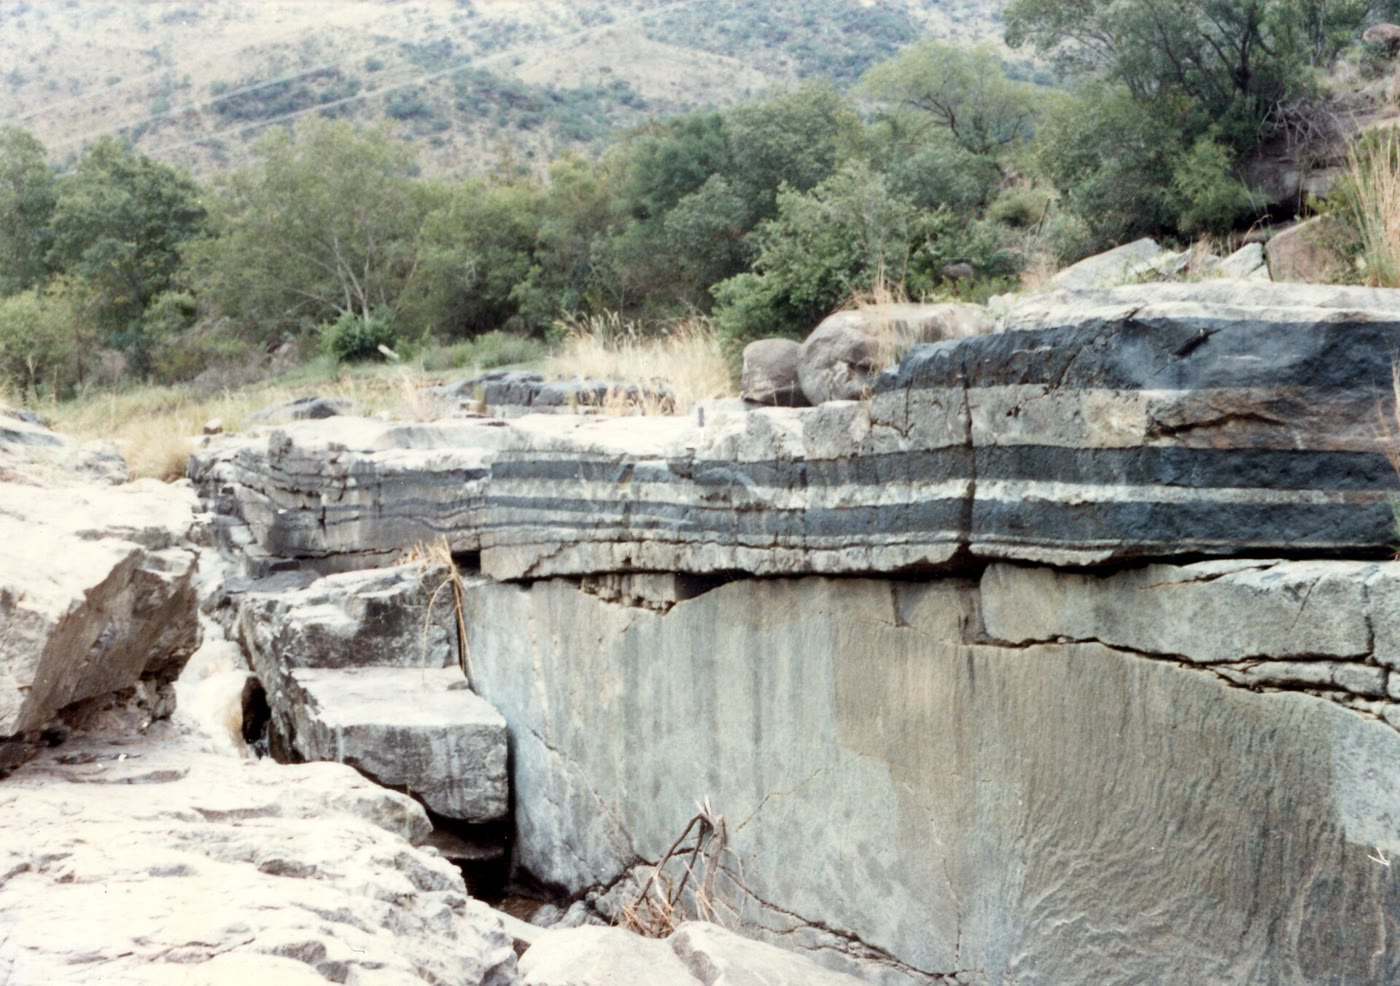
\includegraphics[height=5.2cm]{images/book4/b2-bushveld-chromitite.jpg}
\end{minipage}\hfill
\begin{minipage}[t]{0.42\linewidth}\vspace{0pt}\centering
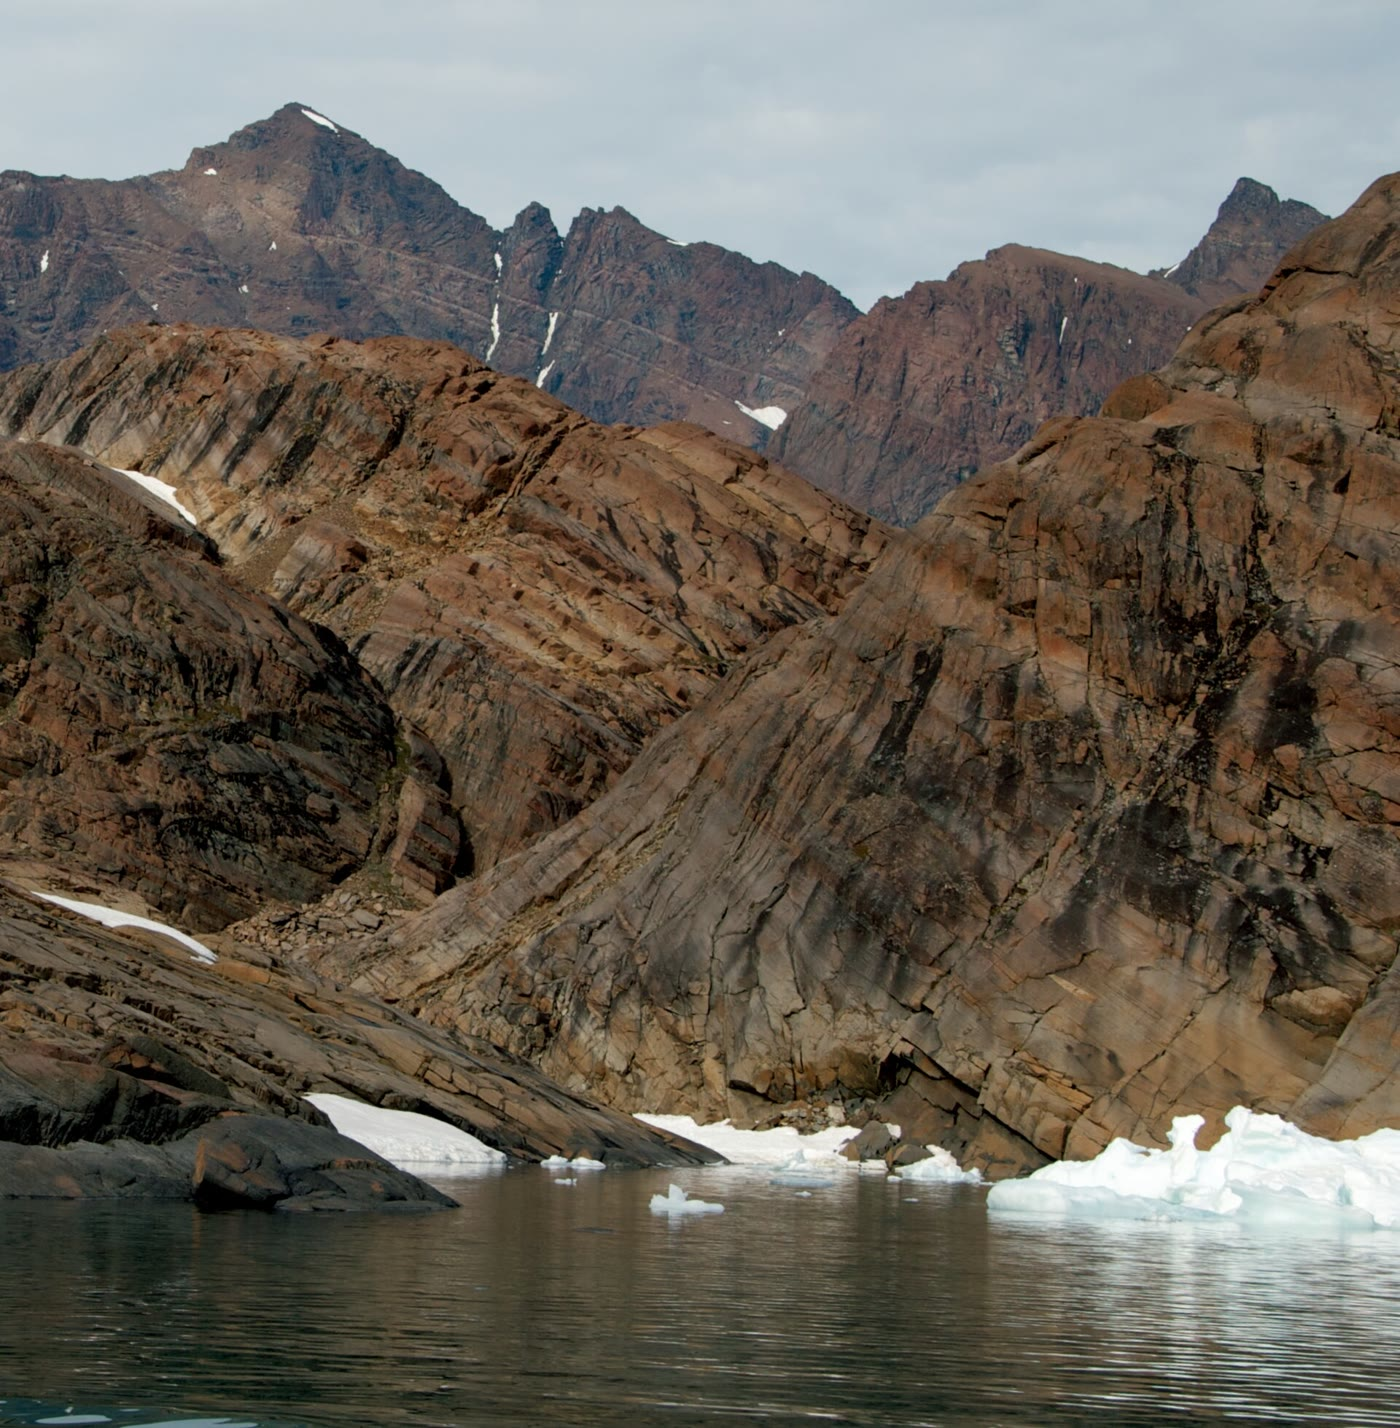
\includegraphics[height=5.2cm]{images/book4/b2-skaergaard-layering.jpg}
\end{minipage}
\par\smallskip{\small Left: black chromitite and grey anorthosite layers of the
Critical Zone of the Bushveld Complex, South Africa (Kevin Walsh, CC BY 2.0).
Right: the layered gabbros of the Middle Zone of the Skaergaard intrusion, East
Greenland, inclined from upper left to lower right (C. Tegner, CC BY 4.0).}
\end{omfigure}

\section{Open systems}\label{sec:b2:magmatic-differentiation:open}

A \omterm{def:b2:magma-emplacement:magma}{magma} chamber is seldom closed. New \omterm{def:b2:magma-emplacement:magma}{magma} arrives from below, and the walls of the
chamber are rocks that the \omterm{def:b2:magma-emplacement:magma}{magma} can heat, melt and dissolve.

\begin{definition}[Magma mixing; crustal assimilation; AFC]
\label{def:b2:magmatic-differentiation:open}
\emph{Magma mixing}\index{magma mixing} is the blending of two \omterm{def:b2:magma-emplacement:magma}{magmas} of different
compositions into one. \emph{Crustal assimilation}\index{crustal assimilation} is the
incorporation of crustal rock into a \omterm{def:b2:magma-emplacement:magma}{magma}, by melting and dissolution of the wall
rock or of blocks fallen into it. \emph{Assimilation--fractional
crystallisation}\index{assimilation--fractional crystallisation} (AFC) is their
combination in one chamber: the \omterm{def:b2:magma-emplacement:magma}{magma} crystallises, and the latent heat released
melts and assimilates the wall rock.
\end{definition}

\begin{proposition}[Mixing is linear in concentrations]\label{prop:b2:magmatic-differentiation:mixing}
A mixture of a mass fraction $s$ of \omterm{def:b2:magma-emplacement:magma}{magma} A and $1-s$ of \omterm{def:b2:magma-emplacement:magma}{magma} B has every
concentration $C = sC_A + (1-s)C_B$: on any diagram of one concentration against
another, mixtures lie on the straight segment from A to B, and the lever rule gives
$s$.
\end{proposition}

\begin{proof}
Each element is conserved: $C(m_A + m_B) = m_AC_A + m_BC_B$; divide by $m_A + m_B$.
\end{proof}

Mixing and crystal removal both draw straight lines on \omterm{def:b2:magmatic-differentiation:harker}{Harker diagrams}; isotope
ratios tell them apart. Crystallisation does not change an isotope ratio, while
mixing with a rock of different ratio does, along the hyperbola of
\cref{ch:b2:isotope-geochemistry}. A rise of $^{87}$Sr/$^{86}$Sr with silica in a
volcanic suite is therefore the mark of assimilation.

\begin{proposition}[Assimilation with fractional crystallisation]
\label{prop:b2:magmatic-differentiation:afc}
A \omterm{def:b2:magma-emplacement:magma}{magma} crystallises crystals with bulk partition coefficient $D$ for an element
and assimilates wall rock of concentration $C_a$ at a rate $r$ times the rate of
crystallisation ($r \ne 1$). With $F$ the mass of \omterm{def:b2:magma-emplacement:magma}{magma} relative to its initial
mass and $z = (r + D - 1)/(r - 1)$,
\[
\frac{C}{C_0} = F^{-z} + \frac{r}{r - 1 + D}\,\frac{C_a}{C_0}\,\bigl(1 - F^{-z}\bigr).
\]
For $r = 0$ this is the Rayleigh law. The isotope ratio of the element in the \omterm{def:b2:magma-emplacement:magma}{magma}
is the mean of that of the initial \omterm{def:b2:magma-emplacement:magma}{magma} and that of the wall rock, weighted by the
two terms of this sum.
\end{proposition}

\begin{proof}
Per unit initial mass, when a mass $\mathrm dm_c$ crystallises, a mass
$r\,\mathrm dm_c$ is assimilated and the \omterm{def:b2:magma-emplacement:magma}{magma} mass changes by $\mathrm dM =
-(1-r)\,\mathrm dm_c$. The element balance is $\mathrm d(MC) = rC_a\,\mathrm dm_c -
DC\,\mathrm dm_c$. Expanding the left side and replacing $\mathrm dm_c$ by
$-\mathrm dM/(1-r)$,
\[
M\frac{\mathrm dC}{\mathrm dM} = -C - \frac{rC_a - DC}{1-r}
= \frac{(r - 1 + D)\,C - rC_a}{1 - r} = -z\,\bigl(C - C^*\bigr),
\qquad C^* = \frac{rC_a}{r - 1 + D}.
\]
So $\mathrm d(C - C^*)/(C - C^*) = -z\,\mathrm dM/M$, and $C - C^*$ is proportional
to $M^{-z}$; with $C = C_0$ at $M = 1$, $C = C^* + (C_0 - C^*)F^{-z}$, which is the
formula. For $r = 0$, $z = 1 - D$ and $C^* = 0$. The atoms that come from the
initial \omterm{def:b2:magma-emplacement:magma}{magma} obey the same equation with $C_a = 0$, so their concentration is
$C_0F^{-z}$; the rest come from the wall: hence the weighting of the isotope ratios.
\end{proof}

DePaolo gave these equations in 1981, and they are the standard model of a \omterm{def:b2:magma-emplacement:magma}{magma}
contaminated on its way through the crust. They hide a thermal constraint. The heat
to assimilate rock comes from the latent heat of the crystals: heating crust from
150 to \qty{1150}{\celsius} takes about \qty{1}{kJ/g}, melting it \qty{300}{J/g},
while crystallising \omterm{def:b2:magma-emplacement:magma}{magma} gives about \qty{400}{J/g}; so some \qty{3.25}{g} of
\omterm{def:b2:magma-emplacement:magma}{magma} must crystallise for each gram of rock assimilated, and $r$ is well below 1.
Wilcox made the same calculation for Parícutin: his \qty{25.4}{g} of quartz
monzonite, taken at about \qty{200}{\celsius}, needed some \qty{31350}{J} to be
heated to \qty{1100}{\celsius} and melted, the heat of crystallising about
\qty{85}{g} of plagioclase, far more than the \qty{12.5}{g} of crystals his mass
balance removed. The erupted \omterm{def:b2:magma-emplacement:magma}{magma} could not have paid for its own assimilation:
the heat must have come from a larger body of \omterm{def:b2:magma-emplacement:magma}{magma} than the one that erupted,
crystallising out of sight (\cref{exo:b2:magmatic-differentiation:11}).
% ledger: depaolo81:afc, white09:afc-heat, wilcox54:heat, wilcox54:mass-balance

\begin{omfigure}
\centering
\begin{tikzpicture}
\begin{axis}[omrecord, name=left, width=0.47\linewidth, height=5.4cm,
  xmin=0.3, xmax=1, ymin=0.3, ymax=1.05, x dir=reverse,
  xlabel={magma remaining $F$}, ylabel={Sr: $C/C_0$},
  tick label style={font=\scriptsize}, label style={font=\small}]
\addplot[thick, black] table[x=F, y=srC_r0] {figdata/out/bachelor-2-differentiation-afc.dat};
\addplot[thick, blue!70!black] table[x=F, y=srC_r02] {figdata/out/bachelor-2-differentiation-afc.dat};
\addplot[thick, red!70!black] table[x=F, y=srC_r05] {figdata/out/bachelor-2-differentiation-afc.dat};
\end{axis}
\begin{axis}[omrecord, at={(left.east)}, anchor=west, xshift=1.7cm,
  width=0.47\linewidth, height=5.4cm,
  xmin=0.3, xmax=1, ymin=0.703, ymax=0.716, x dir=reverse,
  xlabel={magma remaining $F$}, ylabel={$^{87}$Sr/$^{86}$Sr},
  y tick label style={/pgf/number format/fixed, /pgf/number format/precision=3},
  legend style={font=\scriptsize, at={(0.03,0.97)}, anchor=north west},
  tick label style={font=\scriptsize}, label style={font=\small}]
\addplot[thick, black] table[x=F, y=iso_r0] {figdata/out/bachelor-2-differentiation-afc.dat};
\addlegendentry{$r = 0$}
\addplot[thick, blue!70!black] table[x=F, y=iso_r02] {figdata/out/bachelor-2-differentiation-afc.dat};
\addlegendentry{$r = 0.2$}
\addplot[thick, red!70!black] table[x=F, y=iso_r05] {figdata/out/bachelor-2-differentiation-afc.dat};
\addlegendentry{$r = 0.5$}
\end{axis}
\end{tikzpicture}
\par\smallskip{\small Assimilation with \omterm{def:b2:magmatic-differentiation:crystallisation}{fractional crystallisation} for strontium
($D = 1.5$, wall rock with half the strontium of the \omterm{def:b2:magma-emplacement:magma}{magma} and
$^{87}$Sr/$^{86}$Sr = 0.7200, \omterm{def:b2:magma-emplacement:magma}{magma} 0.7035; illustrative values). Left: the
concentration falls faster as the assimilation rate $r$ rises, since the wall rock brings
less strontium and more crystals form for the same $F$. Right: the isotope
ratio, unchanged by crystallisation alone ($r = 0$), climbs towards that of the wall.}
\end{omfigure}

\section{Reading zoned crystals}\label{sec:b2:magmatic-differentiation:zoning}

\begin{definition}[Compositional zoning]\label{def:b2:magmatic-differentiation:zoning}
A crystal of a solid solution shows \emph{compositional zoning}\index{compositional
zoning} when its composition varies from core to rim, recording the changing liquid
from which successive layers grew. Zoning is \emph{normal} when the rim is richer in
the low-temperature component (sodium in plagioclase), \emph{reverse} when it is
richer in the high-temperature one, and \emph{oscillatory} when it alternates.
\end{definition}

A zoned crystal is \omterm{def:b2:magmatic-differentiation:crystallisation}{fractional crystallisation} caught in the act: its core did not
re-equilibrate with the later liquid. The figure below computes, on Bowen's loop,
the plagioclase growing from a liquid of \qty{50}{\percent} anorthite. In
equilibrium the crystals stay homogeneous and end at \qty{50}{\percent}; in perfect
\omterm{def:b2:magmatic-differentiation:crystallisation}{fractional crystallisation} each new layer is in equilibrium with an ever more sodic
liquid, and the rim of the last crystals is nearly pure albite. Normal zoning, from
calcic core to sodic rim, is what Bowen's series predicts for a cooling \omterm{def:b2:magma-emplacement:magma}{magma}. A reverse
zone, a calcic band outside a sodic one, says that the crystal was suddenly bathed in
a hotter or more calcic liquid: often the arrival of new \omterm{def:b2:magma-emplacement:magma}{magma}, mixing in the
chamber.
% ledger: bowen13:plagioclase, earle:bowen (Book 2)

\begin{omfigure}
\centering
\begin{tikzpicture}
\begin{axis}[omrecord, width=0.78\linewidth, height=6cm,
  xmin=0, xmax=1, ymin=0, ymax=90,
  xlabel={fraction of the liquid crystallised},
  ylabel={anorthite (\unit{\percent}, molecular)},
  legend style={font=\scriptsize, at={(0.02,0.02)}, anchor=south west},
  tick label style={font=\scriptsize}, label style={font=\small}]
\addplot[very thick, red!70!black] table[x=x, y=an_frac] {figdata/out/bachelor-2-differentiation-zoning.dat};
\addlegendentry{fractional: layer forming}
\addplot[thick, gray, densely dotted] table[x=x, y=an_liq_frac] {figdata/out/bachelor-2-differentiation-zoning.dat};
\addlegendentry{fractional: liquid}
\addplot[very thick, blue!70!black, dashed] table[x=x, y=an_eq] {figdata/out/bachelor-2-differentiation-zoning.dat};
\addlegendentry{equilibrium: crystals}
\end{axis}
\end{tikzpicture}
\par\smallskip{\small Plagioclase crystallising from a liquid of \qty{50}{\percent}
anorthite, computed on the loop of Bowen (1913). In \omterm{def:b2:magmatic-differentiation:crystallisation}{fractional crystallisation} the
successive layers of the crystals, from core (left) to rim (right), grow ever more
sodic, and the liquid reaches albite when about \qty{82}{\percent} has crystallised; in
\omterm{def:b2:magmatic-differentiation:crystallisation}{equilibrium crystallisation} the crystals stay uniform and end with the composition of
the liquid they came from.}
\end{omfigure}

\begin{inthelab}[Reading zoned crystals]
Petrologists read zoning first between crossed polars, where the zones of a
plagioclase go extinct at slightly different angles and appear as concentric bands.
They then measure it: an electron microprobe (\cref{ch:b2:field-lab-methods-2})
analyses spots a few micrometres across along a traverse from core to rim, and maps
of calcium and sodium show the zones directly. From such a profile they compute the
composition of the liquid each zone grew from, with the loop of the figure above or
with partition coefficients, and they count the reverse zones as the number of
recharges of the chamber. \omterm{def:b2:elements-in-the-earth:trace}{Trace elements} measured along the same traverse by laser
ablation, and isotope ratios measured zone by zone, separate crystallisation, mixing
and assimilation in the history of a single crystal.
\end{inthelab}

\section{Exercises}

\begin{exercise}[$\star$]\label{exo:b2:magmatic-differentiation:1}
Use Bowen's measurements on the plagioclases (solidus / liquidus, \unit{\celsius}):
An$_{100}$ 1550 / 1550; An$_{83.3}$ 1465 / 1521; An$_{66.7}$ 1372 / 1490; An$_{50}$
1287 / 1450; An$_{33.3}$ 1205 / 1394; An$_{20}$ liquidus 1334; An$_{11.1}$ liquidus
1265, and interpolate linearly between neighbouring points. A liquid of
\qty{50}{\percent} anorthite cools in equilibrium. (a) At what temperature does it
begin to crystallise, and what is the composition of the first crystal? (b) At
\qty{1394}{\celsius}, what are the compositions of the liquid and of the crystals,
and what mass fraction has crystallised (use mole fractions as if they were mass
fractions)? (c) What is the composition of the last drop of liquid?
\end{exercise}
% ledger: bowen13:plagioclase

\begin{exercise}[$\star$]\label{exo:b2:magmatic-differentiation:2}
A gabbroic \omterm{def:b2:magmatic-differentiation:cumulate}{cumulate} contains \qty{50}{\percent} plagioclase, \qty{35}{\percent}
clinopyroxene and \qty{15}{\percent} olivine. With the partition coefficients
(olivine / clinopyroxene / plagioclase) Sr 0.000063 / 0.157 / 2.7, Zr 0.00068 /
0.195 / 0.001 and Rb 0.000044 / 0.0033 / 0.025, compute the bulk partition
coefficient of each element, and say which is compatible.
\end{exercise}
% ledger: white07:kd-basalt

\begin{exercise}[$\star$]\label{exo:b2:magmatic-differentiation:3}
The \omterm{def:b2:magmatic-differentiation:cumulate}{cumulate} of \cref{exo:b2:magmatic-differentiation:2} crystallises from a basalt, by \omterm{def:b2:magmatic-differentiation:crystallisation}{fractional crystallisation},
until half of the liquid is left. (a) By what factor has each of Sr, Zr and Rb changed
in the liquid (take the bulk coefficients 1.40, 0.069 and 0.014)? (b) By what factor
has the ratio Zr/Rb changed? Comment with the corollary on ratios.
\end{exercise}
% ledger: white07:kd-basalt

\begin{exercise}[$\star$]\label{exo:b2:magmatic-differentiation:4}
The first lava of Parícutin (February 1943) had \qty{55.04}{\percent} \ce{SiO2},
\qty{5.68}{\percent} \ce{MgO} and \qty{0.85}{\percent} \ce{K2O}; the last (February
1952), 60.07, 3.73 and \qty{1.67}{\percent}. (a) Compute the change of each oxide.
(b) Potash enters none of the crystallising minerals. If it had been concentrated by
\omterm{def:b2:magmatic-differentiation:crystallisation}{fractional crystallisation} alone, what fraction of the liquid would have been left?
(c) Wilcox's mass balance removes only about \qty{12.5}{g} of crystals per
\qty{100}{g} of \omterm{def:b2:magma-emplacement:magma}{magma}. What does the comparison suggest?
\end{exercise}
% ledger: wilcox54:table2, wilcox54:mass-balance

\begin{exercise}[$\star\star$]\label{exo:b2:magmatic-differentiation:5}
Compare fractional and \omterm{def:b2:magmatic-differentiation:crystallisation}{equilibrium crystallisation}: compute $C_L/C_0$ by both laws
(a) for nickel, $D = 5$, when \qty{20}{\percent} of the liquid has crystallised; (b)
for an \omterm{def:b2:elements-in-the-earth:partition}{incompatible element}, $D = 0.01$, when \qty{90}{\percent} has crystallised.
(c) What are the limits of both laws as $F \to 0$? Which law can strip a liquid of a
\omterm{def:b2:elements-in-the-earth:partition}{compatible element} completely?
\end{exercise}

\begin{exercise}[$\star\star$]\label{exo:b2:magmatic-differentiation:6}
(a) Compute the mass percentages of \ce{MgO}, \ce{FeO} and \ce{SiO2} in olivine
Fo$_{80}$, $(\ce{Mg}_{0.8}\ce{Fe}_{0.2})_2\ce{SiO4}$ ($M$ = 40.30, 71.84 and
\qty{60.08}{g/mol}). (b) A basalt with \qty{10.0}{\percent} \ce{MgO} and
\qty{49.0}{\percent} \ce{SiO2} crystallises only this olivine until its liquid has
\qty{8.0}{\percent} \ce{MgO}. What mass fraction of olivine was removed? (c) What
is the silica content of the liquid then?
\end{exercise}

\begin{exercise}[$\star\star$]\label{exo:b2:magmatic-differentiation:7}
For the Skaergaard intrusion, $F = \num{1.091e-7}H^2 - \num{5.9064e-4}H + 0.7678$.
(a) Compute $F$ at $H = 0$, 1000 and \qty{2000}{m}. (b) At what height is $F = 0$?
(c) What fraction of the \omterm{def:b2:magma-emplacement:magma}{magma} had crystallised before the base of the exposed floor
sequence formed, and where could it be?
\end{exercise}
% ledger: tegner23:skaergaard

\begin{exercise}[$\star\star$]\label{exo:b2:magmatic-differentiation:8}
Along the Skaergaard section, the median \omterm{def:b2:magmatic-differentiation:cumulate}{cumulate} holds \qty{177}{ppm} Ni at
$F = 0.70$ (Lower Zone a), \qty{54}{ppm} at $F = 0.29$ (Middle Zone) and
\qty{6.2}{ppm} at $F = 0.17$ (Upper Zone a). (a) Assuming that the \omterm{def:b2:magmatic-differentiation:cumulate}{cumulates} hold
$D$ times the nickel of their liquid and that the liquid follows the Rayleigh law,
compute the apparent $D$ between the first two levels. (b) Do the same between the
last two. (c) What can make the apparent $D$ change?
\end{exercise}
% ledger: data:b4-skaergaard

\begin{exercise}[$\star\star$]\label{exo:b2:magmatic-differentiation:9}
Check Wilcox's answer: \qty{100}{g} of groundmass of the first lava (\ce{SiO2}
55.53, \ce{MgO} 4.66, \ce{K2O} \qty{0.88}{\percent}) plus \qty{25.4}{g} of average
xenolith (72.48, 0.77, 3.64) minus \qty{2.9}{g} of olivine Fo$_{80}$ (39.19, 42.06, 0)
minus \qty{9.6}{g} of plagioclase An$_{70}$ (50.54, 0, 0). (a) What mass remains?
(b) Compute its \ce{SiO2}, \ce{MgO} and \ce{K2O} and compare with the groundmass of
lava 19 (60.16, 3.19 and \qty{1.75}{\percent}). (c) Which oxide fits worst?
\end{exercise}
% ledger: wilcox54:groundmass, wilcox54:xenoliths, wilcox54:mass-balance

\begin{exercise}[$\star\star\star$]\label{exo:b2:magmatic-differentiation:10}
A \omterm{def:b2:magma-emplacement:magma}{magma} assimilates wall rock at $r = 0.2$ while crystallising, with $D_{\ce{Sr}} =
1.5$, $C_a/C_0 = 0.5$, initial $^{87}$Sr/$^{86}$Sr = 0.7035 and wall rock 0.7200.
(a) Compute $z$, $F^{-z}$ and $C/C_0$ at $F = 0.7$. (b) Compare with pure \omterm{def:b2:magmatic-differentiation:crystallisation}{fractional
crystallisation} at the same $F$, and explain the difference with the mass of crystals
formed in each case. (c) Compute the $^{87}$Sr/$^{86}$Sr of the \omterm{def:b2:magma-emplacement:magma}{magma}.
\end{exercise}

\begin{exercise}[$\star\star\star$]\label{exo:b2:magmatic-differentiation:11}
Follow Wilcox's heat budget for Parícutin. (a) How much heat does a gram of quartz
monzonite need to go from 200 to \qty{1100}{\celsius} (heat capacity
\qty{1.1}{J/(g.K)}) and then to melt (\qty{250}{J/g})? (b) How much for
\qty{25.4}{g}? (c) What mass of plagioclase An$_{70}$ (latent heat \qty{370}{J/g})
must crystallise to supply it? (d) Compare with the \qty{12.5}{g} of crystals of the
mass balance, compute the ratio $r$ of assimilation to crystallisation, and say what
this implies.
\end{exercise}
% ledger: wilcox54:heat, white09:afc-heat

\begin{exercise}[$\star\star\star$]\label{exo:b2:magmatic-differentiation:12}
A basalt with \qty{250}{ppm} Ni first crystallises olivine alone ($D = 5$) until
$F = 0.8$, then olivine with plagioclase and clinopyroxene (bulk $D = 1.5$). (a)
Compute the factor by which nickel changes in each stage, and the nickel content of
the liquid at $F = 0.5$. (b) What would a single law with $D = 5$ have predicted?
(c) Explain why the Rayleigh law must be applied in stages.
\end{exercise}

\section{Problem: The intrusion that wrote its own history}

\begin{problem}[{Weekend problem --- from the layers of a gabbro to the fraction of
its magma that was still liquid at the end}]
\label{pb:b2:magmatic-differentiation:1}
An (invented) layered gabbro \omterm{def:b2:magma-emplacement:bodies}{sill} crystallised from a basalt whose \omterm{def:b2:magma-emplacement:aureole}{chilled margin}
gives the parent composition: \ce{SiO2} 49.5, \ce{Al2O3} 16.0, \ce{FeO} 10.0,
\ce{MgO} 9.0, \ce{CaO} 11.5, \ce{Na2O} 2.5, \ce{K2O} \qty{0.30}{\percent};
\qty{150}{ppm} Ni and \qty{80}{ppm} Zr. The lower zone \omterm{def:b2:magmatic-differentiation:cumulate}{cumulates} are made of
\qty{20}{\percent} olivine, \qty{50}{\percent} plagioclase and \qty{30}{\percent}
clinopyroxene; above the level where olivine disappears, of \qty{55}{\percent}
plagioclase and \qty{45}{\percent} clinopyroxene. Take the partition coefficients
(olivine / plagioclase / clinopyroxene) Ni 5.0 / 0 / 2.0 and Zr 0.0007 / 0.001 /
0.195. Mineral compositions (\unit{\percent}): olivine \ce{MgO} 42.06, \ce{CaO} 0,
\ce{Al2O3} 0, \ce{SiO2} 39.19; plagioclase 0, 14.36, 31.70, 50.54; clinopyroxene
16.0, 20.5, 3.0, 51.5. A \omterm{def:b2:magma-emplacement:bodies}{dyke}
of fine-grained rock fed from the chamber when the uppermost layer crystallised has
\ce{SiO2} 50.0, \ce{Al2O3} 14.1, \ce{FeO} 16.7, \ce{MgO} 4.9, \ce{CaO} 7.3,
\ce{Na2O} 3.4, \ce{K2O} \qty{0.75}{\percent} and \qty{188}{ppm} Zr.

\noindent\textbf{Part I --- The partition coefficients of the layers.}
\begin{enumerate}
\item Compute the bulk partition coefficient of nickel in the lower zone.
\item Compute that of zirconium in the lower zone.
\item Compute both in the upper zone.
\item Which element is compatible in each zone? Does nickel stay compatible when
olivine disappears?
\item Which mineral holds most of the zirconium of the \omterm{def:b2:magmatic-differentiation:cumulate}{cumulates}, and why?
\item By what factor does Ni/Zr in the liquid change per halving of $F$ in the lower
zone?
\end{enumerate}

\noindent\textbf{Part II --- Rayleigh curves up the section.}
\begin{enumerate}[resume]
\item What nickel content do you expect in the lowest \omterm{def:b2:magmatic-differentiation:cumulate}{cumulate}, crystallised at
$F = 1$?
\item A lower-zone \omterm{def:b2:magmatic-differentiation:cumulate}{cumulate} higher up holds \qty{190}{ppm} Ni. At what $F$ did it
form?
\item What was then the zirconium content of the liquid?
\item At that $F$, compare the nickel of the liquid given by the fractional and the
equilibrium laws.
\item Olivine disappears at $F = 0.55$. Compute the nickel content of the liquid
there.
\item Compute the nickel of the \omterm{def:b2:magmatic-differentiation:cumulate}{cumulates} formed just below and just above that
level. What feature would a geologist see in the profile?
\item Compute the nickel of the liquid and of the \omterm{def:b2:magmatic-differentiation:cumulate}{cumulate} at $F = 0.40$. Explain
the trend.
\end{enumerate}

\noindent\textbf{Part III --- The mass balance of the last liquid.}
\begin{enumerate}[resume]
\item Write the conservation equation of the method for one oxide, with the masses
$x_{\mathrm{ol}}, x_{\mathrm{pl}}, x_{\mathrm{cpx}}$ removed per \qty{100}{g} of
parent and the \omterm{def:b2:magma-emplacement:bodies}{dyke} as daughter.
\item Write it for \ce{MgO}, \ce{CaO} and \ce{Al2O3}.
\item Solve the $3 \times 3$ system.
\item What fraction of the parent is left as liquid?
\item Check the answer with \ce{SiO2}: recompute the silica of the liquid from the
masses found.
\item Compare the proportions of the minerals removed with the modes of the two
zones.
\item Potash enters none of the minerals: what fraction of liquid does it give?
\end{enumerate}

\noindent\textbf{Part IV --- The fraction of liquid at the top.}
\begin{enumerate}[resume]
\item By what factor had zirconium risen in the liquid when olivine disappeared at
$F = 0.55$? Give the zirconium content then.
\item From the zirconium of the \omterm{def:b2:magma-emplacement:bodies}{dyke}, compute the fraction of liquid remaining when
it formed, applying the upper-zone law from $F = 0.55$.
\item Redo the calculation with a single $D = 0.07$ from the start. Is the answer
sensitive to the details of $D$?
\item Iron rose from 10.0 to \qty{16.7}{\percent} in the liquid while silica barely
changed. Which minerals are responsible, and which kind of magmatic series does
this foreshadow (\cref{ch:b2:magmatic-series})?
\item The uppermost \omterm{def:b2:magmatic-differentiation:cumulate}{cumulates} hold \qty{47}{ppm} Zr. Cumulus crystals alone would hold
$\bar D$ times the zirconium of the liquid; what mass fraction of trapped liquid
(of the \omterm{def:b2:magma-emplacement:bodies}{dyke}'s composition) explains the analysis?
\item State the fraction of the original \omterm{def:b2:magma-emplacement:magma}{magma} still liquid when the uppermost layer
crystallised, the key number of this problem, and compare the three estimates
(major elements, potash, zirconium).
\end{enumerate}
\end{problem}
% ledger: white07:kd-basalt, matzen12:dni
